\documentclass[12pt,letterpaper]{article}
\usepackage{fullpage}
\usepackage[top=2cm, bottom=4.5cm, left=2.5cm, right=2.5cm]{geometry}
\usepackage{amsmath,amsthm,amsfonts,amssymb,amscd}
\usepackage{lastpage}
\usepackage{enumerate}
\usepackage{fancyhdr}
\usepackage{mathrsfs}
\usepackage{xcolor}
\usepackage{graphicx}
\usepackage{setspace}
\usepackage{listings}
\usepackage{minted}
\usepackage{pythonhighlight}
\usepackage{todonotes}
\usepackage{tikz}
\usetikzlibrary{shapes.geometric, arrows}

% \usepackage[margin=1in]{geometry} 
\usepackage{bm}
\newcommand{\matr}[1]{\bm{#1}}     % ISO complying version
\newcommand{\vect}[1]{\bm{#1}}     % ISO complying version
\usepackage[hyphens]{url}
\usepackage[colorlinks]{hyperref}
\usepackage{enumitem}

\makeatletter
\newcommand\RedeclareMathOperator{%
  \@ifstar{\def\rmo@s{m}\rmo@redeclare}{\def\rmo@s{o}\rmo@redeclare}%
}
% this is taken from \renew@command
\newcommand\rmo@redeclare[2]{%
  \begingroup \escapechar\m@ne\xdef\@gtempa{{\string#1}}\endgroup
  \expandafter\@ifundefined\@gtempa
     {\@latex@error{\noexpand#1undefined}\@ehc}%
     \relax
  \expandafter\rmo@declmathop\rmo@s{#1}{#2}}
% This is just \@declmathop without \@ifdefinable
\newcommand\rmo@declmathop[3]{%
  \DeclareRobustCommand{#2}{\qopname\newmcodes@#1{#3}}%
}
\@onlypreamble\RedeclareMathOperator
\makeatother

\DeclareMathOperator{\E}{\mathbb{E}}
\DeclareMathOperator{\V}{\mathbb{V}}
\RedeclareMathOperator{\Pr}{\mathbb{P}}


\hypersetup{%
  colorlinks=true,
  linkcolor=blue,
  linkbordercolor={0 0 1}
}
 
\renewcommand\lstlistingname{Algorithm}
\renewcommand\lstlistlistingname{Algorithms}
\def\lstlistingautorefname{Alg.}

\lstdefinestyle{Python}{
    language        = Python,
    frame           = lines, 
    basicstyle      = \footnotesize,
    keywordstyle    = \color{blue},
    stringstyle     = \color{green},
    commentstyle    = \color{red}\ttfamily
}

\setlength{\parindent}{0.0in}
\setlength{\parskip}{0.05in}

% Edit these as appropriate
\newcommand\course{DS-GA 1008: Deep Learning, Spring 2019}
\newcommand\hwnumber{3}                  % <-- homework number
\newcommand\NetIDa{cz1565}         

\pagestyle{fancyplain}
\headheight 55pt
%\lhead{\NetIDa}
% \lhead{\NetIDa\\\NetIDb}                 % <-- Comment this line out for problem sets (make sure you are person #1)
\chead{\textbf{\Large \course \\ Homework Assignment \hwnumber}\\ 
\textbf{\large Chengze Zuo $|$ cz1565@nyu.edu}}\\

%\rhead{\course \\ \today}
\lfoot{}
\cfoot{}
\rfoot{\small\thepage}
\headsep 1.5em

% tikzlibrary setup
\tikzstyle{startstop} = [rectangle, rounded corners, minimum width=3cm, minimum height=1cm,text centered, draw=black, fill=red!30]
\tikzstyle{io} = [trapezium, trapezium left angle=70, trapezium right angle=110, minimum width=3cm, minimum height=1cm, text centered, draw=black, fill=blue!30]
\tikzstyle{process} = [rectangle, minimum width=3cm, minimum height=1cm, text centered, draw=black, fill=orange!30]
\tikzstyle{process2} = [rectangle, minimum width=3cm, minimum height=2cm, text centered, draw=black, fill=green!30]
\tikzstyle{arrow} = [thick,->,>=stealth]


\begin{document}
\begin{center}
\texttt{If you get, give.  If you learn, teach.  Maya Angelou (1928 - 2014)}
\end{center}
\subsection*{\centering  \href{https://www.overleaf.com/read/bsjxfktnsjsw
}{Read-only Link}
}
\section*{\centering Part I}

\section*{1. Fundamentals}
\subsection*{1.1. Dropout}
\begin{itemize}
    \item[(a)] List the torch.nn module corresponding to 2D dropout. 
    
    Answer: torch.nn.Dropout2d(p=0.5, inplace=False)
    
    \item[(b)] Read on what dropout is and give a short explanation on what it does and why it is useful. 
    
    Answer: Dropout is a technique that aims to reduce overfitting and provides a way of approximately combining many different neural networks together efficiently. The term "dropout" means that the some units in the hidden/input layers would be randomly removed from the neural network during the training time. Each unit would have a fixed probability p (indeendent of other units) representing this unit would be retained or not. Applying dropout to a neural network would amount to sampling a thinned version network from the original large network, where for each training time just one of the thinned version networks would be sampled and trained. The reason why dropout is useful is because it breaks the strong co-adaptions between the units to make dependence between units or the presence of units more unreliable. Randomly removing units during the training time adds "noise" to the network and make units more independent (rely more on themselves). Therefore this technique help reduce the generalization error greatly.
\end{itemize}

\subsection*{1.2 Batch Normalization}
\begin{itemize}
    \item[(a)]What does mini-batch refer to in the context of deep learning?
    
    Answer: The term mini-batch in the context of deep learning is referred as using more than one but less than all the training examples. 
    
    \item[(b)]Read on what batch norm is and give a short explanation on what it does and why it is useful.
    
    Answer: In the deep learning realm, we may refer the term internal covariance shift as the change in the distribution of network activations due to the change in network parameters during training. This effect would be amplified the network goes deeper, thus causing training to be really difficult. Batch normalization (aka batch norm) aims to solve (or at least alleviate) this problem, and therefore speed up training neural nets. It is a method of reparametization. The batch norm being useful is because firstly it reduces the internal covariance shift to make sure each layer inputs has desired distribution (fixed mean and variance), which would accelerate training the whole network. Moreover, the batch norm makes it possible to use saturating nonlinearities by preventing the network from getting stuck in the saturated mode. Thirdly, batch norm makes the neural network more resilliant to the parameter scale so that it will reduce the dependence of gradients on the parameter scale and of their initial values. Finally, batch norm would enable higher learning rate since it stablizes the learning and could regularize the model, thus reducing the need for dropout (Because the network no longer produces deterministic value for a given training example). 
\end{itemize}
\section*{2. Language Modeling}
\begin{itemize}
    \item[(a)]Go through the code and draw a block diagram / flow chart (see this tutorial) which highlights the main interacting components, illustrates their functionality, and provides an estimate of their computational time percentage (rough profiling).
    
    Answer: 
    For the sake of simplicity, we would illustrate the training process concretely. It would be similar for the evaluation and prediction phase as well.\\
    1)Prepare: Prepare word dictionary/dorpus and arrange the corpus into training, validation and testing set (in data.py).\\
    2)Batchify: This phase batchifies training corpuse(set) into a set of batches. Starting from sequential data, batchify arranges the dataset into columns. For every batch training, send one batch to the model.
    3)RNN: Based on the model type that is selected, the training phase begins. Each batch training the model computes the output and final hidden state. The output is used to compute the loss while the hidden state will be detached for every next batch training. The reason to do this is because we want the backpropogation through time is only computed through this current batch instead of to the start of the whole training set. During each batch training, the \textbf{torch.nn.utils.clip\_grad\_norm\_} would be used to the gradient clipping to reduce the issue of the exploding gradient. The model.py contains parts including encoder, dropout, rnn and decoder. 
    
    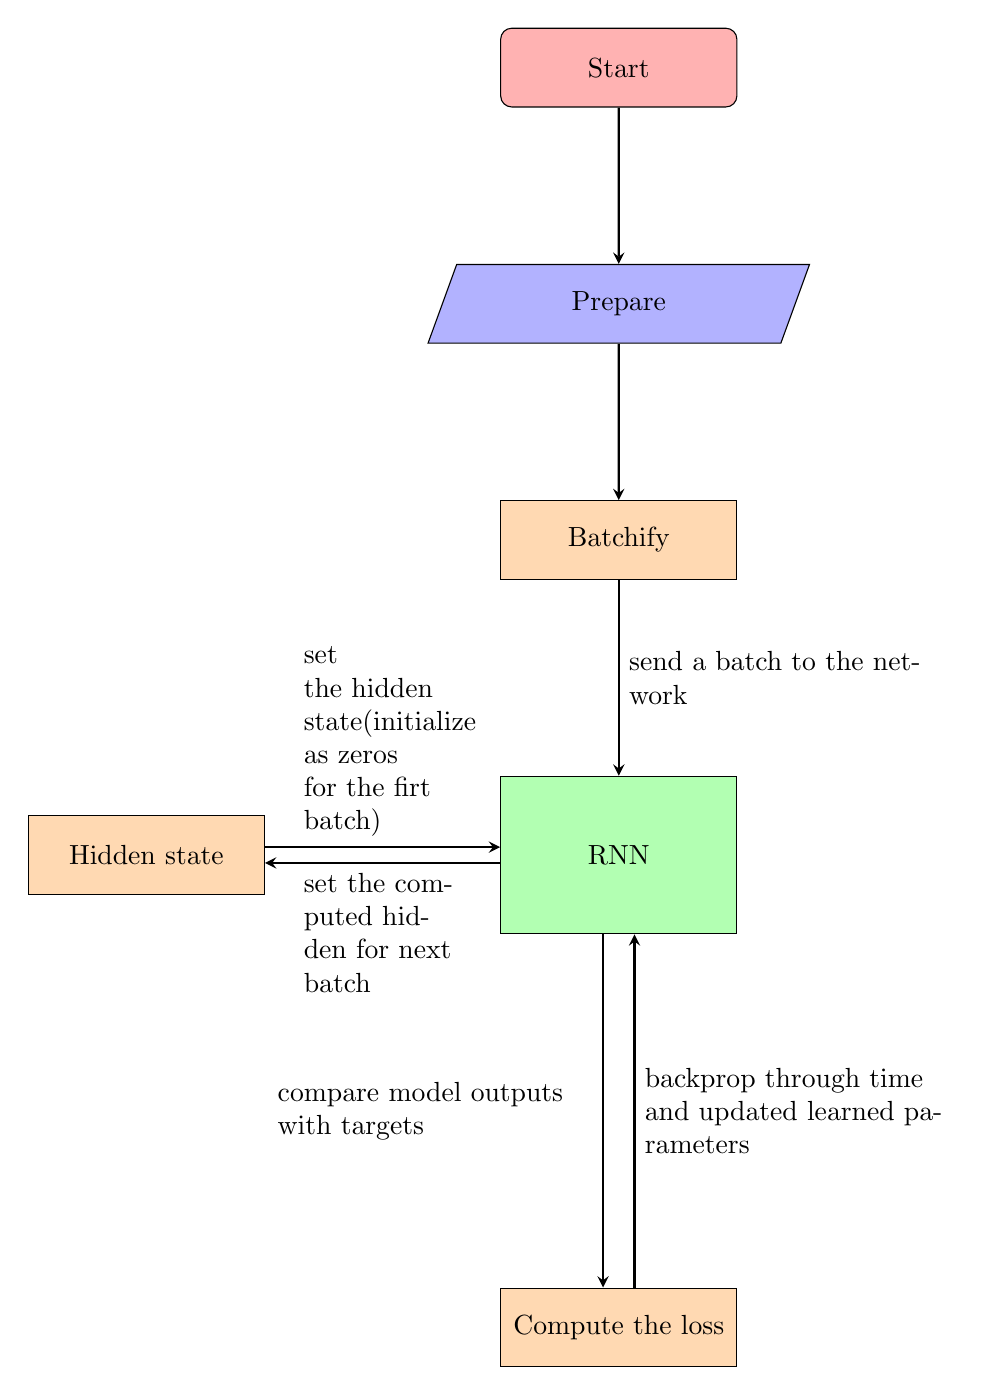
\begin{tikzpicture}[node distance=2cm]
        \node (start) [startstop] {Start};
        \node (prepare) [io, below of=start, yshift=-1cm, text width=2cm] {Prepare};
        \node (batch) [process, yshift=-1cm, below of=prepare] {Batchify};
        \node (train) [process2, below of=batch, yshift=-2cm] {RNN};
        \node (hidden) [process, left of=train, xshift=-4cm, text width=2cm] {Hidden state};
        \node (loss) [process, below of=train, yshift=-4cm] {Compute the loss};
        
        \draw [arrow] (start) -- (prepare);
        \draw [arrow] (prepare) -- (batch);
        \draw [arrow] (batch) -- node[anchor=west, text width=4cm]{send a batch to the network} (train);
        
        \draw [arrow] ([yshift=0.1cm]hidden.east) -- node[anchor=south, text width=2cm] {set the hidden state(initialize as zeros for the firt batch)} ([yshift=0.1cm]train.west);
        
        \draw [arrow] ([yshift=-0.1cm]train.west) -- node[anchor=north, text width=2cm] {set the computed hidden for next batch} ([yshift=-0.1cm]hidden.east);
        
        \draw [arrow] ([xshift=-0.2cm]train.south) -- node[anchor=east, text width=4cm] {compare model outputs with targets} ([xshift=-0.2cm]loss.north);
        
        \draw [arrow] ([xshift=0.2cm]loss.north) -- node[anchor=west, text width = 4cm]{backprop through time and updated learned parameters} ([xshift=0.2cm]train.south);
        % downward is NORTH
        
        
    \end{tikzpicture}
    
    \item[(b)]Find and explain where and how the back-propagation through time (BPTT) takes place (you may need to delve into PyTorch source code).
    
    Answer: In the main.py the BPTT happens in line:
    \begin{python}
        loss.backward()
    \end{python}
    
    From the PyTorch source code, the computational graph on which the backward() is called actually forms from here:
    \begin{python}
    if batch_sizes is None:
        result = _impl(input, hx, self._flat_weights, self.bias, self.num_layers,
         self.dropout, self.training, self.bidirectional, self.batch_first)
    else:
        result = _impl(input, batch_sizes, hx, self._flat_weights, self.bias,
         self.num_layers, self.dropout, self.training, self.bidirectional)
    \end{python}
    For some reason, I could not find the C/C++ source code module\\ \textbf{torch.\_C.\_VariableFunctions} which owns the source implementation for rnn\_tanh function.
    
    Depends on different types of RNNs (many to one, many to many, one to many, encoder/decoder), the computation of the overall loss might be a little bit different, but the overall thought process would be similar. Suppose we have have recurrent neural network that have a pair of input/output at every time step in sequence. We unroll the network, compute and accumulate the loss across each time step, which is $\textbf{L} = \sum \textbf{L}^{(t)}$. After computing the accumulated loss, the loss is backpropogated through the whole network to the start. For a given model parameter, e.g. weight matrix, it is shared by each RNN unit across all time steps. Therefore, during the backpropagation through time, the gradient w.r.t the weight matrix could be summed across all time steps (all instances of the network). After that, the model parameter (weight matrix) is updated given by specified learning rate.
    
    \item[(c)]Describe why we need the repackage hidden(h) function, and how it works.
    
    Answer: Every time we start a new batch and train them on the network, we would use the hidden state that was produced from the last batch, so during the BPTT the loss would be propagated through this batch only instead of across all batches. Therefore, we need to the detach the item of the hidden state into a new Tensor and treat this new Tensor as the new initial hidden state for next batch training.
    
    How it works: if the hidden state is a Tensor object, the repackage\_hidden function will detach that hidden state item and return a new Tensor object with same item that was detached. If the hidden state is an iterable object of Tensors, then we recursively call the repackage\_hidden function and store each detach hidden state in to tuple.
    
    \item[(d)]Why is there a --tied (tie the word embedding and softmax weights) option?
    
    Answer: The --tied option would enforce the dimension of input embedding matrix equals to the dimension of output embedding matrix. By tying these two embedding matrix, this would lead to an improvement in terms of the perplexity of the language model. The joint embedding would have similar way to the output embedding compared to the input embedding of the untied model. Thus the model would have better performance in terms of the similar words or interchangeable words. Last but not least, by tying the two embedding matrices, this would significantly reduce the number of parameters that need be to learned, therefore improving the model with respect to preventing from overfitting and accelerating training.
    
    \item[(e)]Compare LSTM and GRU performance (validation perplexity and training time) for different values of the following parameters: number of epochs, number of layers, hid- den units size, input embedding dimensionality, BPTT temporal interval, and non- linearities (pick just 3 of these parameters and experiment with 2-3 different values for each).
    
    Answer: \\
    1)By comparing the LSTM and GRU with different epochs, I chose epochs with 2 and 4 respectively (number of layers is 2). For epoch number 4, GRU obtains higher validation perplexity while the LSTM would train longer; Turning the epochs to 2, both of the two networks are trained faster w.r.t training time in total, but compared to same type of model with 4 epochs, each epoch cost a little bit more time. Besides, GRU still has higher validation perplexity.\\
    2)By comparing the LSTM and GRU with different number of layers, I chose nlayers with 1 and 2 (with 4 epochs to train). As the number of layer increases, the models both have longer training time (for each epoch and in total) and bigger training perplexity. For 2-layer model, epochs with more than 4 may be needed because the ppl might continues to decrease. In a nutshell, GRU would have larger validation perplexity but less training time compared to the LSTM (both for 1 layer and 2 layers).
    3)By comparing the LSTM and GRU with different number of hidden units, I chose nhid 450, 650 and 850 for 1 layer and 4 epochs. For one-layer (default is 2) model, as the number of hidden units increases, the training time decreases a slight bit, but not obviously, and the validation perplexity also decreases a little bit (for same type of model). Usually GRU would end up with higher validation perplexity compared with LSTM.
    
    \item[(f)]Why do we compute performance on a test set as well? What is this number good for?
    
    Anwser: After we evaluate the performance on the training and validation test, we could possibly select the model that has best-performance. But this does not guarantee that our model would perform well on new unseen data. Therefore, we also need to compute the performance on a test set, and moreover, evaluating this number is good for obtaining the best(lowest) generalization error for the model that we could possibly do.
\end{itemize}
\end{document}